% ============================================================================
% ONR FY2027 Young Investigator Program (YIP), Technical Proposal (Volume 1)
% NOFO N0001426SF004 (posted 17 Aug 2026, file FY27_YIP_NOFO_N0001426SF004__003.pdf)
% Due 30 Oct 2026, 5:00 PM Eastern, via Grants.gov (NOFO p. 27).
%
% Format (NOFO pp. 15-16): 8.5 x 11 in, 1 in margins, single-spaced,
% Times New Roman 12 pt, technical proposal limited to 20 pages.
% Excluded from the limit (NOFO p. 16): cover page, table of contents, full CV,
% data management plan, letters of support, cited references, current and
% pending support.
% Required sections and order (NOFO pp. 18-20): Cover Page; Table of Contents;
% Technical Approach (with Future Naval Relevance, Project Schedule and
% Milestones, Goals and Benchmarks, Gold Standard Science); Management
% Approach; Principal Investigator Qualifications; Principal Investigator's CV;
% Letter(s) of Support; Responsibility; Data Management Plan (2 pages max).
% Field 9 (NOFO p. 20) takes the references as a separate PDF; they are also
% printed at the end of this file for review.
%
% Sources: the AFOSR A.2.c white paper (afosr-yip-white-paper-a2c.tex) for the
% method, hypotheses, and simulation; the FLAIME DOE proposal
% (genesis-mission-proposal/flaime-genesis-proposal.tex) for the staged
% specimens, feedstock route, CALPHAD features, and the scandium objective.
%
% Page numbering: pages that count toward the 20-page limit are numbered
% 1, 2, ...; excluded parts carry their own prefixes (CV, L, D, S, R) so the
% count is visible at a glance.
%
% Red [TODO Sterling: ...] markers are guesses or facts not yet confirmed.
%
% Build: xelatex onr-yip-technical-proposal.tex (twice)
% ============================================================================

\documentclass[12pt,letterpaper]{article}

\usepackage[margin=1in]{geometry}
\usepackage{iftex}
\ifPDFTeX
  \usepackage[T1]{fontenc}
  \usepackage[utf8]{inputenc}
  \usepackage{mathptmx}
\else
  \usepackage{fontspec}
  \IfFontExistsTF{Times New Roman}
    {\setmainfont{Times New Roman}}
    {\setmainfont{TeX Gyre Termes}}
\fi
\usepackage{microtype}

\setlength{\parindent}{0pt}
\setlength{\parskip}{5pt plus 2pt minus 1pt}
\setlength{\textfloatsep}{10pt plus 2pt minus 2pt}

\usepackage{graphicx}
\usepackage{xcolor}
\usepackage{tikz}
\usetikzlibrary{positioning,arrows.meta,fit}
\usepackage{array}
\usepackage{booktabs}
\usepackage{tabularx}
\usepackage{pdfpages}
\usepackage[labelfont=bf,labelsep=period,skip=4pt]{caption}
\usepackage{xurl}
\usepackage[colorlinks=true,linkcolor=blue!70!black,citecolor=blue!70!black,
  urlcolor=blue!70!black]{hyperref}

\usepackage{titlesec}
\titleformat{\section}{\normalfont\normalsize\bfseries}{\thesection.}{0.5em}{}
\titlespacing*{\section}{0pt}{10pt plus 2pt minus 2pt}{2pt}
\titleformat{\subsection}{\normalfont\normalsize\bfseries}{\thesubsection}{0.5em}{}
\titlespacing*{\subsection}{0pt}{8pt plus 2pt minus 2pt}{1pt}
\titleformat{\subsubsection}[runin]{\normalfont\normalsize\bfseries}{}{0pt}{}[.]
\titlespacing*{\subsubsection}{0pt}{5pt plus 2pt minus 1pt}{0.5em}

\pagestyle{plain}
\newcommand{\todo}[1]{\textcolor{red}{[TODO Sterling: #1]}}
\hyphenation{re-POW-DER AMA-ZE-MET}

\newcommand{\BudgetTotal}{747,651}
\newcommand{\BudgetYearOne}{248,959}
\newcommand{\MTDCYearOne}{140,298}
\newcommand{\FAYearOne}{72,253}
\newcommand{\BuildsYearOne}{28}
\newcommand{\BudgetYearTwo}{248,828}
\newcommand{\MTDCYearTwo}{151,728}
\newcommand{\FAYearTwo}{78,140}
\newcommand{\BuildsYearTwo}{29}
\newcommand{\BudgetYearThree}{249,864}
\newcommand{\MTDCYearThree}{152,036}
\newcommand{\FAYearThree}{78,299}
\newcommand{\BuildsYearThree}{26}

\begin{document}

% ===========================================================================
% Cover page (excluded from the page limit)
% ===========================================================================
\pagenumbering{roman}
\begin{titlepage}
\begin{center}
{\Large\bfseries Technical Proposal\par}
\vspace{10pt}
{\large\bfseries Cost-Aware Selection of Experiments for Printable,\\
Corrosion-Resistant High-Strength Aluminum Alloys\par}
\vspace{10pt}
Office of Naval Research (ONR)\\
Fiscal Year 2027 Young Investigator Program (YIP)
\end{center}
\vspace{12pt}
\renewcommand{\arraystretch}{1.25}
\begin{tabular}{@{}>{\bfseries\raggedright\arraybackslash}p{1.95in}>{\raggedright\arraybackslash}p{4.3in}@{}}
NOFO number & N0001426SF004 \\
Title & Cost-Aware Selection of Experiments for Printable, Corrosion-Resistant
  High-Strength Aluminum Alloys \\
Prime applicant & Brigham Young University (BYU), Provo, Utah \\
Subawardees & None \\
ONR S\&T Focus Areas & Primary: Manufacturing (Integrated Manufacturing and
  Sustainment Technologies). Secondary: Materials and Electronics
  (Sustainable and Operationally Robust Materials). \\
ONR program & Materials \& Processes for Additive Manufacturing, Code 332
  (Dr.~Charles Fisher) \todo{confirm after his reply} \\
Technical contact & Sterling G.\ Baird, Ph.D., Assistant Professor,
  Department of Mechanical Engineering, Brigham Young University, 350 EB,
  Provo, UT 84602. Phone (801) 422-5344. Email
  \href{mailto:sterling.baird@byu.edu}{sterling.baird@byu.edu} \\
Administrative and business contact & \todo{name, title, address, phone,
  and email of the BYU Research Administration officer who signs as the
  Authorized Organization Representative} \\
Period of performance & Base period only, 36 months: 1 April 2027 to
  31 March 2030. No option periods. \\
Requested amount & \$\BudgetTotal{} total: \$\BudgetYearOne, \$\BudgetYearTwo,
  and \$\BudgetYearThree{} in the three 12-month periods \todo{final figures
  from BYU Research Administration} \\
\end{tabular}
\end{titlepage}

% ===========================================================================
% Table of contents (excluded from the page limit)
% ===========================================================================
\setcounter{page}{2}
\setcounter{tocdepth}{2}
\tableofcontents
\clearpage

% ===========================================================================
% Pages 1 to N count toward the 20-page limit
% ===========================================================================
\pagenumbering{arabic}

\section{Technical Approach}

\subsection{Problem and objectives}

Developing a new alloy for laser powder bed fusion (LPBF) runs through a chain
of steps: a thermodynamic calculation, powder production, printed test
specimens, microscopy, and property tests. For a part that will serve at sea,
the property tests include corrosion tests, and the longest of those run for
weeks. The costs of the steps differ greatly. A thermodynamic calculation
takes minutes, a printed build takes days including turnaround, and a
corrosion exposure takes weeks. Experimental campaigns often send each
candidate through the whole chain, spending much of the budget on full tests
of candidates that a cheap early measurement could have ruled out.
Computational campaigns often work as a funnel: many simulations, then a few
candidates passed on to experiments. If the simulation misses a physical
effect, the funnel discards good candidates before any experiment can catch
the error.

High-strength aluminum alloys show this cost problem clearly. Most of them,
such as 7075, crack as they solidify during LPBF, so printed aluminum parts
mostly use the casting alloy AlSi10Mg~\cite{martin2017}. Additions that refine
the grains, such as zirconium, can prevent the cracking~\cite{martin2017}, but
each change in composition changes how the alloy solidifies, and the laser
settings must be tuned again~\cite{debroy2018}. The rapid solidification also
changes how the alloy corrodes (Section~\ref{sec:naval-al}), so corrosion data
for a wrought alloy do not carry over to its printed version. Each new
composition therefore repeats a long test program, corrosion tests included,
before a printed part can go on a ship or an aircraft.

This project asks a basic question. When the steps of a materials workflow
differ in cost by orders of magnitude, and results arrive at different times,
how should one choose the next measurement and the next candidate? The aim is
to reach a set of qualified properties, including resistance to corrosion in
seawater, at the lowest total cost. The project has five objectives:
\begin{enumerate}\setlength{\itemsep}{0pt}
\item Extend a cost-aware search method that learns from partial results to
several competing objectives: free of cracks and pores, strong, ductile, and
resistant to corrosion in chloride solutions.
\item Extend it to many experiments in progress at once, with results that
return at different times.
\item Demonstrate both on a physical workflow for printable high-strength
aluminum alloys, from powder to tensile and corrosion tests.
\item Test whether the method's stated confidence in a candidate matches what
the printer, the test frame, and the corrosion tests later show.
\item Measure how well a one-hour electrochemical screen predicts corrosion
tests that take days to weeks, so that the long tests run only where they can
change a decision.
\end{enumerate}

\subsection{Printed aluminum in naval service}
\label{sec:naval-al}

Aluminum alloys are light and resist general corrosion, so the Navy uses them
where weight and speed matter: in ship structures~\cite{golumbfskie2016} and
in aircraft~\cite{dursun2014}. Their behavior in seawater has shaped Navy
maintenance. The aluminum-magnesium (5000-series) alloys used in
superstructures become sensitized in service: time at warm temperatures
forms a nearly continuous network of the beta phase
(Al$_3$Mg$_2$) along grain boundaries. The beta phase is anodic to the
aluminum matrix, and in seawater under load it gives a path for stress
corrosion cracking, which has plagued the superstructures of Navy ships for
more than a decade~\cite{golumbfskie2016}. In 2012 Naval Sea Systems Command
(NAVSEA) told Congress that superstructure cracking on the cruisers would
cost \$270 million to repair~\cite{insidedefense2012}. Both Littoral Combat
Ship variants also use 5000-series alloys, and the rate of beta-phase
precipitation can vary by up to 40 times between plate lots bought to the
same specification~\cite{navsea2018sttr}. The lesson is that an alloy's
corrosion behavior after years of service depends on details of its
microstructure that short tests may not reveal.

Printing changes those details. In printed AlSi10Mg, corrosion attacks
selectively along the borders of the melt pools, where the microstructure is
coarser and the difference in potential between the silicon and aluminum
phases is larger~\cite{cabrini2016,revilla2017}. Annealing at high temperature
removes that selective attack but brings galvanic coupling with coarse
silicon particles~\cite{cabrini2016}. Printed 2024 forms a different main
second phase (Al$_2$Cu) than the wrought alloy (Al$_2$CuMg)~\cite{gharbi2018},
and second phases set much of the corrosion behavior of aluminum
alloys~\cite{birbilis2005}. For printable high-strength compositions
the results are mixed. Printed Al-Mn-Cr-Zr resisted sodium chloride solution
and natural seawater better than printed AlSi10Mg~\cite{linder2024}, and
zirconium let 5083 print without cracks and made it more resistant than
printed AlSi10Mg and wrought 5083 in 168-hour immersion
tests~\cite{zhou2021}. Heat treatment, on the other hand, worsened the
corrosion of printed Al-Mn-Mg-Sc-Zr~\cite{zhang2023}. A 2026 review found
that some studies report better corrosion resistance than conventional
alloys and others worse, and that the effects of single microstructural
features are hard to isolate~\cite{alhashem2026}. Each composition and heat
treatment needs its own tests.

Corrosion tests follow the same cost pattern as the rest of the workflow. A
cyclic polarization scan in sodium chloride solution takes about an hour and
gives the potential at which pits start and the potential below which they
stop growing~\cite{astmG61}. Intergranular corrosion tests take 6 to 24
hours of exposure, followed by metallography or
weighing~\cite{astmG110,astmG67,cabreracorrea2022}. Salt-spray exposures and alternate-immersion
stress corrosion tests run for days to weeks~\cite{astmB117,astmG44}. The
search can therefore treat corrosion the way it treats cracking and strength:
a cheap screen for many candidates and long tests for a few. The cheap screen
can mislead, though. In printed Al-Mg-Sc-Zr aged at 150\,\textdegree{}C,
cyclic polarization and impedance in sodium chloride solution were unchanged,
yet the beta phase covered most grain boundaries and made the alloy
susceptible to intergranular corrosion~\cite{cabreracorrea2023}. Knowing when
the screen can be trusted is part of the research.

Supply adds one more objective. Scandium is used mainly in aerospace alloys,
and the United States imports all of the scandium it uses; none was mined or
recovered domestically in 2025~\cite{usgs2026sc}. Zirconium also refines the
grains of printed aluminum~\cite{martin2017}. The search will carry scandium
content as an objective to minimize, as in the simulation of
Section~\ref{sec:prelim}.

\subsection{Scientific concepts}

The search method treats the workflow as a network of linked
models~\cite{astudillo2021}. Each step gets its own statistical model, a
Gaussian process, which predicts the outputs of that step together with their
uncertainty. The models are linked in the same order as the steps
(Fig.~\ref{fig:network}), so the outputs of one step are inputs to the next
and uncertainty carries through the whole network. Because each step has its
own model, the network learns from partial results, and a candidate can stop
at any step. Buathong et al.\ added a cost-aware rule to this
network~\cite{buathong2024}. For each possible experiment, the rule estimates
how much the result is expected to improve the search, divides that by the
experiment's cost, and runs the best one.

Calculation of phase diagrams (CALPHAD) in Thermo-Calc and
pycalphad~\cite{andersson2002,otis2017} supplies the physics at the first
step. It gives the freezing range, the phases expected during
solidification, and an index of how prone the alloy is to cracking as it
solidifies~\cite{kou2015}. It also gives the second phases that may form
along grain boundaries, which matter for corrosion~\cite{birbilis2005}. These outputs enter the statistical models as
inputs with learned weights, so the search can discount any of them that
proves uninformative. The calculations run continuously on BYU
high-performance computing, and each new result is available to the next
decision.

\begin{figure}[t]
\centering
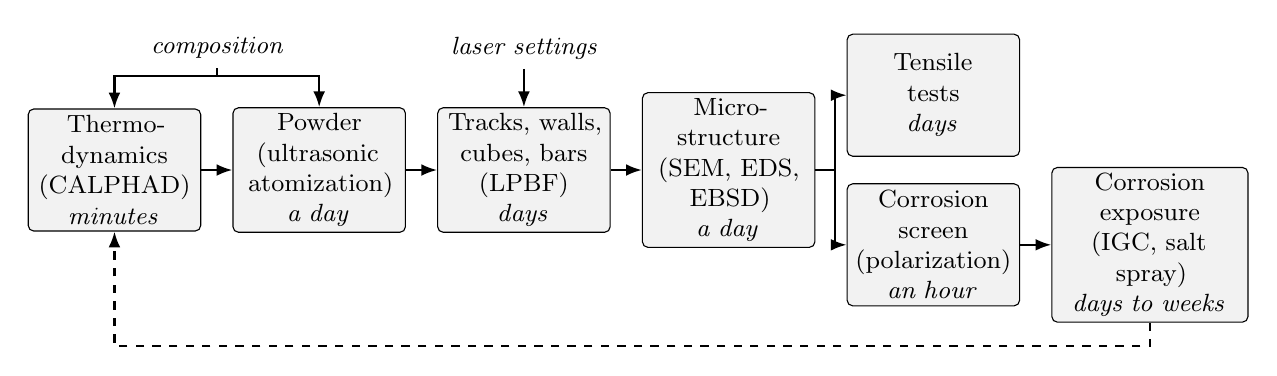
\begin{tikzpicture}[
  font=\small,
  box/.style={draw, rounded corners=2pt, fill=black!5, align=center,
    text width=2.05cm, minimum height=1.55cm, inner sep=2pt},
  arr/.style={-{Latex[length=2mm]}, thick},
  input/.style={font=\small\itshape, align=center}
]
\node[box] (s1) at (0,0) {Thermo-\\dynamics\\(CALPHAD)\\\textit{minutes}};
\node[box] (s2) at (2.6,0) {Powder\\(ultrasonic\\atomization)\\\textit{a day}};
\node[box] (s3) at (5.2,0) {Tracks, walls,\\cubes, bars\\(LPBF)\\\textit{days}};
\node[box] (s4) at (7.8,0) {Micro-\\structure\\(SEM, EDS,\\EBSD)\\\textit{a day}};
\node[box] (s5) at (10.4,0.95) {Tensile\\tests\\\textit{days}};
\node[box] (s6) at (10.4,-0.95) {Corrosion\\screen\\(polarization)\\\textit{an hour}};
\node[box, text width=2.35cm] (s7) at (13.15,-0.95) {Corrosion\\exposure\\(IGC, salt spray)\\\textit{days to weeks}};
\foreach \a/\b in {s1/s2, s2/s3, s3/s4, s6/s7} \draw[arr] (\a) -- (\b);
\draw[arr] (s4.east) -- ++(0.25,0) |- (s5.west);
\draw[arr] (s4.east) -- ++(0.25,0) |- (s6.west);
\node[input] (comp) at (1.3,1.55) {composition};
\draw[arr] (comp.south) -- ++(0,-0.1) -| (s1.north);
\draw[arr] (comp.south) -- ++(0,-0.1) -| (s2.north);
\node[input] (laser) at (5.2,1.55) {laser settings};
\draw[arr] (laser) -- (s3);
\draw[arr, dashed] (s7.south) -- ++(0,-0.3) -| (s1.south);
\end{tikzpicture}
\caption{The workflow as linked models, with typical times per result in
italics (builds include turnaround at the user facility). Composition enters
at the first two steps and laser settings at the third. After microscopy the
network branches to tensile tests and to corrosion tests (IGC, intergranular
corrosion). Dashed arrow: each result updates the models, which choose the
next experiments and steps by expected gain per cost.}
\label{fig:network}
\end{figure}

\subsection{Comparison with other approaches}

To our knowledge, neither a multi-objective nor an asynchronous version of
cost-aware, partial-evaluation optimization of linked models has been
developed, and none has been demonstrated on a physical alloy workflow.
Published tests of the linked-model methods use test functions and
simulators~\cite{astudillo2021,buathong2024}. Multi-stage Bayesian
optimization for self-driving laboratories was tested on synthetic and
retrospective data with one objective~\cite{torresi2026}. Cost-aware batch
optimization of refractory alloys treats measurements of unequal cost as
separate sources rather than linked steps, in a computational
campaign~\cite{alvi2026}. Closed-loop campaigns on printed alloys use one
model and a fixed set of measurements~\cite{talbot2026}. Printable
high-strength aluminum alloys have been designed computationally and then
printed as single compositions~\cite{thapliyal2020,taheri2025}. Standard multi-objective Bayesian
optimization handles competing properties and batches~\cite{daulton2021} but
treats the whole chain as one costly experiment. Corrosion studies of printed
aluminum characterize one alloy at a time with a fixed set of
tests~\cite{cabrini2016,linder2024,zhou2021}. Autonomous and high-throughput
corrosion work has used a scanning droplet cell to screen coatings and has
run fast screens before slower, more thorough tests~\cite{decost2022,sur2023},
but without deciding, candidate by candidate, when a long test is worth its
cost. This project combines the
linked network, the cost per step, several objectives including corrosion,
and results that arrive out of order, and tests the combination on real
builds.

\subsection{Preliminary results}
\label{sec:prelim}

Since the lab started at BYU in December 2025, we have set up a CALPHAD
workflow on BYU high-performance computing. We have also completed a
powder-to-part demonstration on a baseline aluminum alloy. Atomized powder,
LPBF builds, scanning electron microscopy (SEM) and energy-dispersive X-ray
spectroscopy (EDS) results, and tensile data are in hand.
\todo{add a quarter-page figure of the baseline powder (SEM), a printed cube,
and the tensile curve; 9 pages of the 20-page limit are still free.}

% Fig. 2 redraws the synthetic network from the MS&T26 talk
% (benchmarks/bofn-prelim/explain/frames/00-network.png); functions and costs
% are in benchmarks/bofn-prelim/README.md.
\begin{figure}[t]
\centering
\resizebox{\textwidth}{!}{%
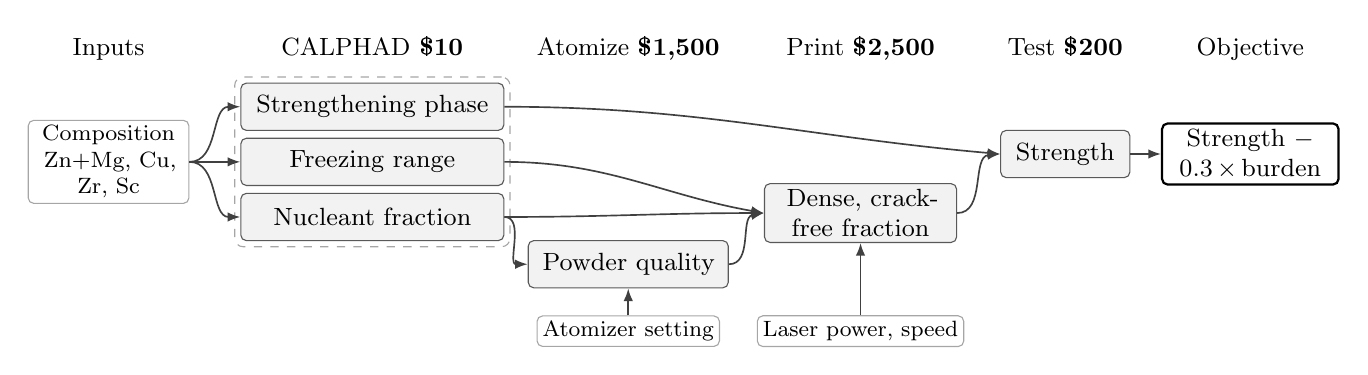
\begin{tikzpicture}[
  font=\small,
  nd/.style={draw=black!65, rounded corners=2pt, fill=black!5, align=center,
    minimum height=0.6cm, inner sep=2pt},
  inp/.style={draw=black!35, rounded corners=2pt, align=center,
    font=\footnotesize, inner sep=2pt},
  hd/.style={font=\small, anchor=base},
  e/.style={-{Latex[length=1.6mm]}, black!75, semithick}
]
\foreach \x/\t in {0.95/Inputs, 4.3/{CALPHAD \textbf{\$10}},
  7.55/{Atomize \textbf{\$1,500}}, 10.5/{Print \textbf{\$2,500}},
  13.1/{Test \textbf{\$200}}, 15.45/Objective}
  \node[hd] at (\x,2.75) {\t};
\node[inp, text width=1.9cm] (c) at (0.95,1.4) {Composition\\Zn+Mg, Cu,\\Zr, Sc};
\node[nd, text width=3.2cm] (s) at (4.3,2.1) {Strengthening phase};
\node[nd, text width=3.2cm] (f) at (4.3,1.4) {Freezing range};
\node[nd, text width=3.2cm] (g) at (4.3,0.7) {Nucleant fraction};
\node[draw=black!35, dashed, rounded corners=3pt, inner sep=2pt,
  fit=(s)(f)(g)] {};
\node[nd, text width=2.4cm] (q) at (7.55,0.1) {Powder quality};
\node[nd, text width=2.3cm] (r) at (10.5,0.75) {Dense, crack-\\free fraction};
\node[nd, text width=1.5cm] (u) at (13.1,1.5) {Strength};
\node[nd, draw=black, thick, fill=white, text width=2.1cm] (o) at (15.45,1.5)
  {Strength $-$\\0.3\,$\times$\,burden};
\node[inp] (a) at (7.55,-0.75) {Atomizer setting};
\node[inp] (l) at (10.5,-0.75) {Laser power, speed};
\foreach \n in {s,f,g} \draw[e] (c.east) to[out=0, in=180] (\n.west);
\draw[e] (s.east) to[out=0, in=175] (u.west);
\draw[e] (f.east) to[out=0, in=170] (r.west);
\draw[e] (g.east) to[out=0, in=180] (r.west);
\draw[e] (g.east) to[out=0, in=180] (q.west);
\draw[e] (q.east) to[out=0, in=190] (r.west);
\draw[e] (r.east) to[out=0, in=185] (u.west);
\draw[e] (u) -- (o);
\draw[e] (a) -- (q);
\draw[e] (l) -- (r);
\end{tikzpicture}}
\caption{Synthetic workflow used for Fig.~\ref{fig:sim}: a hand-written
function for each box and a rough total cost (time, materials, supplies) for
each step. Burden is a penalty on scarce elements such as scandium. The
nucleant (Zr, Sc) cuts cracking, an effect the CALPHAD crack screen does not
see.}
\label{fig:synth}
\end{figure}

% Results: benchmarks/bofn-prelim/README.md (kappa = 1 headline, 20 seeds).
\begin{figure}[t]
\centering
\begin{minipage}[c]{3.1in}
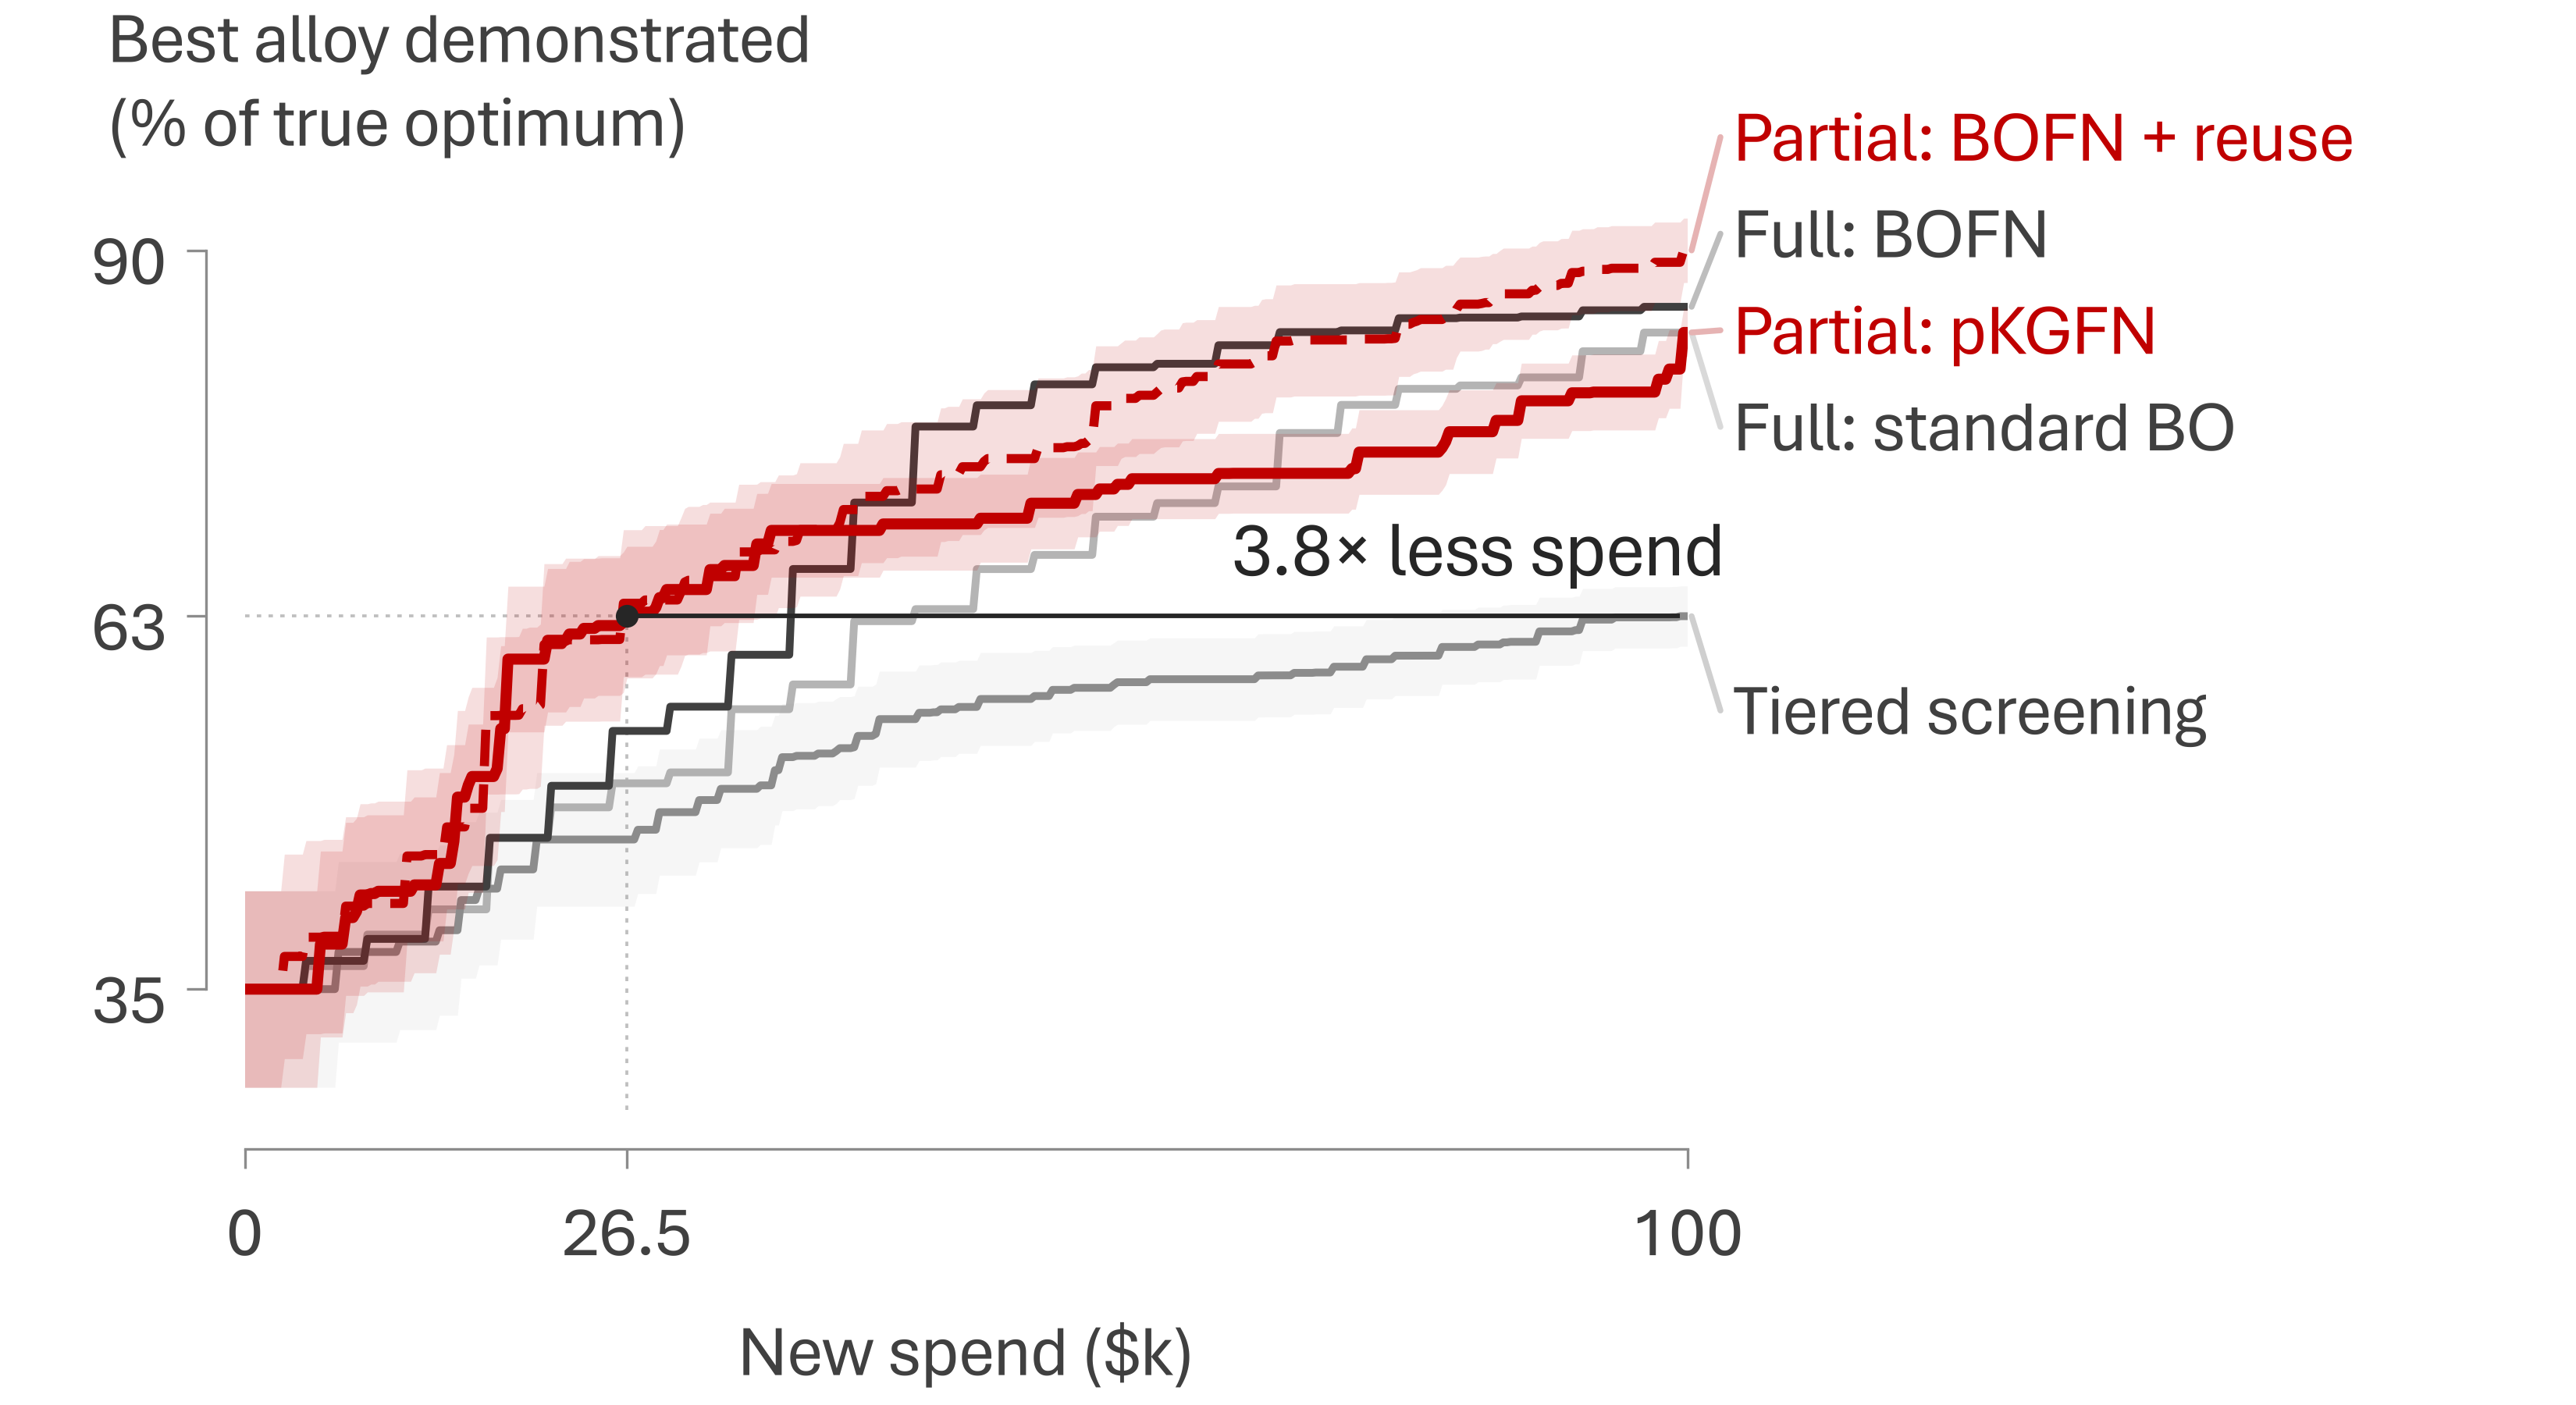
\includegraphics[width=\linewidth]{../../benchmarks/bofn-prelim/bofn_best_vs_spend_k1_partial_vs_full.png}
\end{minipage}\hfill
\begin{minipage}[c]{3.25in}
\caption{Best result found versus spend in simulations where the CALPHAD
crack screen ignores zirconium (means of 20 campaigns, $\pm$1 standard
error). Red searches choose the next step; gray ones follow a fixed order.
pKGFN is the cost-aware method~\cite{buathong2024} and BOFN the linked-model
method~\cite{astudillo2021}; reuse reprints earlier powders.}
\label{fig:sim}
\end{minipage}
\end{figure}

We also simulated the cost-aware method on the steps of
Fig.~\ref{fig:network} up to the tensile test (Figs.~\ref{fig:synth}
and~\ref{fig:sim}). With the crack screen ignoring zirconium, screening and
then tuning the process stalled at 63\% of the optimum after \$100,000. The
cost-aware search, and a simpler one that reused powders, reached that level
after about \$26,500 (3.8 times less spend; 90\% confidence interval 2.0 to
5.7). Searches that ran every candidate through the full chain caught up
later, and screening kept pace when its physics was right. The simulation is
hand-built and noise-free, with one objective, no corrosion branch, and one
experiment at a time, so it does not test the advances proposed here. It does
show that choosing the step, not just the candidate, can matter when the
physics model is incomplete.

\subsection{Method advances}

\subsubsection{Advance 1: several competing objectives}
The published cost-aware method optimizes a single objective. A printed
aluminum part for a ship or an aircraft must balance freedom from cracks and
pores, strength, ductility, and corrosion resistance, with no weighting known
in advance. We will extend the cost-aware rule to several objectives. The
expected improvement in one objective will be replaced by the expected growth
of the set of best trade-offs (the Pareto front), measured by hypervolume as
in multi-objective Bayesian optimization~\cite{daulton2021}, and divided by
cost as before. The difficulty is that each cheap measurement informs some
objectives strongly and others weakly. Single laser tracks show cracking well
but say little about strength or corrosion, and a polarization scan says much
about pitting and nothing about strength. The rule has to account for that
through the network. We will derive the rule, check it against brute-force
estimates on small problems, and measure its computing time on BYU
high-performance computing.

\subsubsection{Advance 2: results that arrive out of order}
The published method chooses one experiment at a time and waits for its
result. In this workflow a build holds many specimens, microscopy results
arrive days after printing, salt-spray exposures run for weeks, and
thermodynamic calculations finish in minutes. We will extend the rule to
batches whose results arrive at different times, so that new experiments are
chosen while others are still pending. Pending experiments will enter the
models as simulated results drawn from the current predictions, a standard way
to avoid choosing the same experiment twice~\cite{snoek2012}. We will also
test how stable the choices are when a late result contradicts early ones.
For example, a cube that looked dense in a photograph may show cracks under
the microscope, or an alloy that passed the polarization screen may fail the
salt-spray test.

\subsubsection{Advance 3: a physical workflow with a corrosion branch}
We will demonstrate both advances on a physical workflow that branches after
microscopy: specimens go to tensile tests, or to the corrosion screen and, for
selected candidates, to longer corrosion tests (Fig.~\ref{fig:network}). The
demonstration includes real build-to-build scatter, outputs computed from
microscopy images, and two inputs (composition and laser settings) that enter
at different steps. CALPHAD outputs will enter the models as physics inputs.
This also tests how much incomplete physics helps, since standard CALPHAD
calculations ignore the very fast cooling of the melt pool~\cite{debroy2018}.

\subsubsection{Advance 4: checking what the screens discard}
A cheap screen saves money only if it does not discard good candidates, and
the sensitized Al-Mg-Sc-Zr example in Section~\ref{sec:naval-al} shows that a
screen can also pass bad ones~\cite{cabreracorrea2023}. Each
round, the search will send a small random share of the candidates it would
stop, about one in ten, on to the next step anyway. These audited candidates
measure how often each screen is wrong, and they keep the models from learning
only from candidates that the screens favored.

\subsection{Hypotheses and rejection criteria}

\textbf{H1 (cost).} The cost-aware, multi-objective search that handles
pending results will reach a target set of trade-offs at lower total cost
than standard batch multi-objective Bayesian optimization, which carries
every candidate through the full chain. H1 will be rejected if, across
matched campaigns with the same budget, the median cost to reach the target is
not lower than the full-chain baseline's.

\textbf{H2 (calibration).} The predicted probabilities that a candidate will
be dense, crack-free, and close to its intended composition will match the
observed rates on held-out builds. H2 will be rejected if observed success
rates differ from predicted probabilities by more than 10 percentage points.

\textbf{H3 (physics inputs).} Using CALPHAD outputs as physics inputs will
improve that calibration over models trained on data alone. H3 will be
rejected if the physics inputs do not reduce calibration error on held-out
builds.

\textbf{H4 (pending results).} Choosing new experiments while others are
pending will reach the target in less calendar time than waiting for each
batch to finish, at equal spend. H4 will be rejected if, in median calendar
time, the version that works around pending results is no faster than the
version that waits.

\textbf{H5 (corrosion screen).} Pitting and repassivation potentials from the
one-hour screen, together with composition and microstructure, will predict
which candidates pass the longer intergranular and salt-spray tests. H5 will
be rejected if, among tested candidates (audited ones included), those that
the model ranks in the top half pass the long tests no more often than those
in the bottom half.

The targets, baselines, budgets, and number of matched campaigns will be
fixed and posted before each test starts \todo{confirm a public
pre-registration site, e.g., OSF}. H1 and H4 are tested first on simulated
and retrospective benchmarks, where many matched campaigns are affordable, and
then in live campaigns, where only a few are.

\subsection{Research plan}

\subsubsection{Task 1: methods (Ph.D. student 1)}
Derive and implement the multi-objective rule (Advance 1), the rule for
pending results (Advance 2), and the audit of screened-out candidates
(Advance 4). Build simulated benchmarks that extend Fig.~\ref{fig:synth}
with noise, several objectives, a corrosion branch, and delays drawn from our
measured turnaround times. Build a retrospective benchmark from the aluminum
data already in hand and the data that Task 2 adds each year.

\subsubsection{Task 2: experimental platform (Ph.D. student 2)}
Powder for each candidate will be made in our laboratory. Elemental and
master-alloy feedstock is weighed to 0.1~mg into machined crucibles of
high-purity aluminum, about 100~g per composition, and atomized by an
ultrasonic atomizer (AMAZEMET rePOWDER). Its induction-melting module covers
aluminum alloys and makes four compositions per week. Each round, the search
will choose compositions and laser settings (power, scan speed, and hatch
spacing). LPBF builds will be bought from a University of Utah user facility
at \$800 per build. A first build of each chosen powder holds single laser
tracks (melt-pool size, balling, cracking), thin walls (crack
susceptibility), and 5~mm cubes (density and porosity) at several laser
settings. Powders whose cubes reach 99\% relative density can get a second
build with sub-size tensile bars (ASTM E8/E8M) and corrosion coupons at the
chosen settings. The search decides which powders are printed at all, since
the atomizer makes powder faster than the budget can print it.

Selected cubes will be examined by SEM, by EDS and inductively coupled plasma
mass spectrometry for composition (magnesium and zinc can evaporate during
melting~\cite{debroy2018}), and by electron backscatter diffraction (EBSD)
for grain size and shape, at BYU. Replicate tracks and cubes at fixed settings
will measure build-to-build scatter. Image analysis scripts will turn
micrographs into porosity, crack length, and grain size with stated
uncertainty.

Corrosion tests follow the same staging. Polished cube faces get
open-circuit potential and cyclic polarization scans in 3.5~wt\% sodium
chloride solution, as in studies of printed Al-Mg-Sc-Zr~\cite{cabreracorrea2023},
on a potentiostat dedicated to the loop, so that the search can schedule the
screen like any other step. The scans follow ASTM G61~\cite{astmG61}, which
is written for iron-, nickel-, and cobalt-based alloys, and the intergranular
tests below were written for wrought products, so the project will report
how each behaves on printed aluminum. Candidates that
the search selects get intergranular corrosion tests~\cite{astmG110}, with the
mass-loss test after a sensitizing heat treatment for alloys rich in
magnesium~\cite{astmG67}. The leading candidates get neutral salt-spray
exposure~\cite{astmB117} at an outside test laboratory. Stress corrosion tests
under alternate immersion~\cite{astmG44}, which take weeks under load, are
left to Navy laboratories for the final candidates
(Section~\ref{sec:naval}).

The alloy space starts from aluminum with zirconium or scandium, which
refine the grains and prevent cracking~\cite{martin2017,thapliyal2020}, and
adds copper, magnesium, zinc, manganese, and chromium for strength. Copper
and zinc raise strength, but the phases they form act as local cathodes or
anodes in chloride solutions~\cite{birbilis2005}, which is the kind of
trade-off the multi-objective rule must manage \todo{confirm the alloy
families and the element ranges to search}.

\subsubsection{Task 3: live campaigns and hypothesis tests (both students)}
Run live campaigns in which the search chooses each experiment and step.
Compare it on equal budgets with random selection and with standard batch
multi-objective Bayesian optimization over the full chain. Test H2 and H3 on
held-out builds, H5 on the audited and selected candidates, and H1 and H4 in
matched campaigns.

\subsubsection{Task 4: release and transition}
Release the software, data, and models each year (Section~\ref{sec:dmp}).
Write a short guide for applying the method to other alloys, printers, and
test sequences, aimed at Navy laboratory and depot engineers. Share the
corrosion data for the final candidates with Navy materials engineers, who
can decide which candidates merit stress corrosion and service-environment
tests.

\subsection{Expected results and new knowledge}

If successful, the project will produce:
\begin{enumerate}\setlength{\itemsep}{0pt}
\item The first cost-aware method of this kind for competing properties and
staggered results.
\item A measured answer to how much a staged, cost-aware search saves over
full-chain testing on a real alloy workflow.
\item Calibrated predictions of printability for high-strength aluminum
compositions, with the value of incomplete CALPHAD physics measured.
\item Corrosion data for printed high-strength aluminum compositions, and a
measured link between a one-hour electrochemical screen and tests that take
days to weeks.
\item New printable high-strength aluminum compositions with their laser
settings, tensile properties, and corrosion behavior, and with less scandium
where the trade-offs allow.
\end{enumerate}
Results that reject a hypothesis are also new knowledge. For example, if H1
fails, the data will show which step's cost or noise erased the advantage; if
H5 fails, they will show which microstructural features the screen missed.

\subsection{Future Naval Relevance}
\label{sec:naval}

\textbf{ONR S\&T Focus Areas.} The primary focus area is Manufacturing,
research area Integrated Manufacturing and Sustainment Technologies. The
secondary focus area is Materials and Electronics, research area Sustainable
and Operationally Robust Materials. Within Code 332 the project fits the
program Materials \& Processes for Additive Manufacturing~\cite{onram}. That
program lists five thrusts, including (i) rapid qualification frameworks,
(ii) tailored AM materials and processes, and (v) AM and digital logistics,
and names the challenge to ``develop and validate computational approaches
for AM materials and processes for engineering applications''~\cite{onram}.
The search method is a qualification tool: it decides which test to run next
and states its confidence in the outcome. The aluminum work develops tailored
alloys and laser settings with their corrosion behavior. The open software
lets a site with a printer and a test sequence run the same logic. It also fits two
other Code 332 programs: Corrosion Science and Corrosion Control
Technologies, which notes that machine learning can ``accelerate materials
discovery and predict material life under various environmental
conditions''~\cite{onrcorr}, and Computer-Aided Materials Design, whose
thrusts include high-throughput screening concepts and
informatics~\cite{onrcamd}.

\textbf{Corrosion and sustainment.} The Navy sustains ships and aircraft that
operate in seawater, far from their supply chains, and it is moving printed
metal parts into service. In April 2026, Fleet Readiness Center East
delivered its first printed metal aircraft parts to the fleet, made with
lasers that ``weld thin layers of aluminum powder''; they are
non-flight-critical fittings for the AH-1Z, V-22, and
C-130~\cite{frce2026}. In August 2026, the Navy set out ``a streamlined,
repeatable technical pathway to substitute legacy cast and wrought parts with
3D-printed metallic materials'' for submarines~\cite{navy2026ppd}. The DoD
additive manufacturing strategy notes that printing ``contributes to a
reduced risk of obsolete parts''~\cite{dodam2021}. Corrosion is a known
barrier for aluminum. A 2019 America Makes award on rapid qualification
described the corrosion behavior of printed AlSi10Mg as unique to printing
and not yet well understood. It said this behavior ``creates a roadblock to
DOD adoption of LPBF parts for mission-critical defense systems in
potentially corrosive environments''~\cite{americamakes2019}. ONR's
corrosion program asks for work on the ``corrosion mechanism in additive
manufactured (AM) alloys'' and on feedstock chemistry for ``corrosion
resistance of additive-manufactured alloys''~\cite{onrcorr}. The
sensitization of superstructure alloys shows the cost of learning about
corrosion in service~\cite{golumbfskie2016}. This project addresses these
needs. It will produce printable high-strength aluminum compositions with
measured corrosion behavior, and a method that lowers the cost of qualifying
each new composition by running long tests only where they change a
decision.

\textbf{Supply.} High-strength printable aluminum that needs less scandium
reduces dependence on an element the United States imports
entirely~\cite{usgs2026sc}.

\textbf{Beyond aluminum.} The method needs only a network of steps, their
costs, and their measurements, so it applies to other Navy materials,
printers, and test sequences, including the repair and qualification of
printed steel and nickel parts. A plasma melting module for our atomizer (not
part of this request) would extend the experimental work to refractory alloys.

\textbf{Navy engagement and people.} The PI presented autonomous
experimentation for alloy discovery at the Naval Surface Warfare Center
(NSWC) Carderock Division in October 2026 \todo{confirm after the 14 October
talk, and name any Carderock contacts who agree to be listed}. The PI will
apply to the Summer Faculty Research Program to spend a summer at a Navy
laboratory \todo{confirm; the 2027 application closes 14 December 2026}. The
project will train two Ph.D.\ students and undergraduates in printing,
characterization, corrosion testing, and autonomous experimentation. We will
encourage them to apply to the Naval Research Enterprise Internship Program
and the SMART and NDSEG programs, which the NOFO names as goals of the YIP.

\subsection{Project Schedule and Milestones}

Table~\ref{tab:schedule} lists the schedule by year. The award start date is
1 April 2027.

\begin{table}[h]
\centering
\caption{Schedule and milestones (Y = project year, starting 1 April 2027).}
\label{tab:schedule}
\renewcommand{\arraystretch}{1.15}
\begin{tabularx}{\textwidth}{@{}p{0.4in}>{\raggedright\arraybackslash}X>{\raggedright\arraybackslash}p{2.05in}@{}}
\toprule
\textbf{Year} & \textbf{Work} & \textbf{Milestone (month)} \\
\midrule
Y1 & Derive the multi-objective rule; build simulated and retrospective
benchmarks; set up the corrosion screen and measure its repeatability on the
baseline alloy; replicate builds to measure scatter; automate image analysis.
& M1: scatter measured on baseline alloy (6).\newline M2: corrosion screen
repeatability measured (8).\newline M3: multi-objective rule passes
small-problem checks (9).\newline M4: benchmarks frozen and posted (12). \\
Y2 & Derive the rule for pending results; first live campaign with tensile and
corrosion branches; first intergranular and salt-spray tests; test H2 and H3
on held-out builds. & M5: first live campaign done (18).\newline M6: H2 and H3
tested (22).\newline M7: methods paper and software release 1 (24). \\
Y3 & Matched live campaigns against the full-chain baseline; test H1, H4, and
H5; release software, data, and guide; share corrosion data with Navy
engineers. & M8: matched campaigns done (32).\newline M9: H1, H4, and H5
tested (34).\newline M10: final release and report (36). \\
\bottomrule
\end{tabularx}
\end{table}

\subsection{Goals and Benchmarks}

Table~\ref{tab:goals} lists each goal and the benchmark used to measure
progress. Progress will be reported at each ONR program review.

\begin{table}[h]
\centering
\caption{Goals and the benchmarks that measure them.}
\label{tab:goals}
\renewcommand{\arraystretch}{1.15}
\begin{tabularx}{\textwidth}{@{}>{\raggedright\arraybackslash}p{1.75in}>{\raggedright\arraybackslash}X@{}}
\toprule
\textbf{Goal} & \textbf{Benchmark} \\
\midrule
Multi-objective cost-aware rule & Matches brute-force estimates on small
problems; finds a larger set of trade-offs per dollar than full-chain
multi-objective search on the simulated benchmark. \\
Rule for pending results & Same final quality as the one-at-a-time rule in
less calendar time on the simulated benchmark with measured delays (H4). \\
Calibrated predictions & Observed success rates within 10 percentage points
of predicted probabilities on held-out builds (H2). \\
Physics inputs & Lower calibration error with CALPHAD inputs than without
(H3). \\
Corrosion screen & Top-ranked candidates pass the long corrosion tests more
often than bottom-ranked ones (H5). \\
Lower cost on real builds & Lower median cost to reach the target than the
full-chain baseline in matched live campaigns (H1). \\
New alloys & At least \todo{number} new compositions printed dense and
crack-free, with tensile and corrosion data, beyond the baseline alloy. \\
Open release & Software, data, and models posted each year with tests and
documentation. \\
\bottomrule
\end{tabularx}
\end{table}

\subsection{Gold Standard Science}

Executive Order 14303 lists nine tenets of Gold Standard
Science~\cite{eo14303}. Such science is reproducible, transparent,
communicative of error and uncertainty, collaborative and interdisciplinary,
and skeptical of its findings and assumptions. It is also structured for
falsifiability of hypotheses, subject to unbiased peer review, accepting of
negative results as positive outcomes, and without conflicts of interest. The
plan follows each point. Each hypothesis above has a stated rejection
criterion, and the targets and baselines are fixed before each test. Every
prediction carries an uncertainty, and the calibration tests (H2, H3) check
whether that uncertainty is honest. The audit of screened-out candidates
(Advance 4) tests the screens' own assumptions. Replicate builds measure
scatter so that it is not mistaken for a real effect. Code, data, and models
are released each year so others can rerun every analysis. Results that
reject a hypothesis will be published like any other result. The PI's record
supports this: the PI co-authored a review of self-driving laboratories and
led open benchmark and software projects (see Section~\ref{sec:quals}).

\section{Management Approach}
\label{sec:mgmt}

This is a single-PI project with no co-PIs or subawards. The PI will lead the
method development, set the campaign plans, and supervise all students.
Ph.D.\ student 1 will lead Task 1 (methods, benchmarks, software). Ph.D.\
student 2 will lead Task 2 (powder, builds, microscopy, tensile and corrosion
tests). An undergraduate researcher will help make powder, prepare specimens,
and run the corrosion screen. Both Ph.D.\ students share Task 3, so the
methods are tested on the data they will face.

LPBF builds are bought at a set rate from a University of Utah user facility,
and salt-spray exposures from an outside test laboratory; neither is a
subaward. About 20 builds per year fit the budget. All other work is at BYU:
the PI's atomizer laboratory, the BYU Microscopy Center (SEM, EDS, EBSD), and
BYU high-performance computing. The team meets weekly to review new results
and choose the next experiments. A shared data pipeline records every step,
so the search always sees the latest results. The schedule and milestones are
in Table~\ref{tab:schedule}.

\textbf{Risks and responses.} If the multi-objective rule is too slow to
compute, we will use a cheaper approximation and measure the loss on the
simulated benchmark. If build scatter is large, more replicates will be
added and the scatter will enter the models directly. If a composition cannot
be atomized, the search records the failure as a result, since predicting
which compositions can be made is part of the task. If LPBF turnaround is
slow, the rule for pending results is designed for exactly that case. If the
polarization screen predicts the long corrosion tests poorly (H5 rejected),
the search will rely more on the long tests, at higher cost, and the audited
candidates will show which features the screen missed.

\section{Principal Investigator Qualifications}
\label{sec:quals}

Sterling G.\ Baird received a Ph.D.\ in Materials Science and Engineering
from the University of Utah in August 2023. He has been an Assistant
Professor of Mechanical Engineering at BYU since December 2025, his first
tenure-track position. Before BYU, he was Director of Training and Programs
and then a Principal Investigator and Staff Scientist at the Acceleration
Consortium, University of Toronto, where he built the Acceleration
Consortium's development laboratory, including about \$600,000 of equipment.

The PI's work combines Bayesian optimization with laboratory hardware. He
developed Honegumi, which helps experimentalists set up Bayesian
optimization, consulted for Meta on the version 1.0 release of the Ax
platform, and organized an international Bayesian optimization hackathon. He
co-authored the structural materials section of the \emph{Chemical Reviews}
survey of self-driving laboratories and led a review of low-cost
self-driving laboratories. His graduate work used Bayesian inference with
propagated uncertainty to model grain boundaries. He also designed a
semi-automated induction furnace for temperatures up to 2500\,\textdegree{}C.
At BYU he supervises eight undergraduate researchers and has set up the
CALPHAD workflow and the powder-to-part demonstration described in
Section~\ref{sec:prelim}. \todo{add any corrosion or electrochemistry
experience; if there is none, say how the students will learn the ASTM
corrosion methods, e.g., a BYU colleague's training or a Navy laboratory
visit.} The CV lists all publications and presentations.

% ===========================================================================
% CV (excluded from the page limit)
% ===========================================================================
\clearpage
\newcounter{savedpage}
\setcounter{savedpage}{\value{page}}
\setcounter{page}{1}
\renewcommand{\thepage}{CV-\arabic{page}}
\phantomsection
\addcontentsline{toc}{section}{Principal Investigator's Curriculum Vitae
  (excluded from page limit)}
\IfFileExists{../../bios/baird-CV.pdf}{%
  \includepdf[pages=-,pagecommand={\thispagestyle{empty}}]{../../bios/baird-CV.pdf}%
}{\textbf{Principal Investigator's Curriculum Vitae}\par
  \todo{insert the full CV PDF here.}\clearpage}

% ===========================================================================
% Letter of support (excluded from the page limit)
% ===========================================================================
\setcounter{page}{1}
\renewcommand{\thepage}{L-\arabic{page}}
\phantomsection
\addcontentsline{toc}{section}{Letter of Support (excluded from page limit)}
\begin{center}\textbf{Letter of Support}\end{center}
\todo{insert the signed letter from the BYU official here as a PDF page
(draft in support-letter-draft.md).}
\clearpage

% ===========================================================================
% Responsibility (counts toward the page limit; numbering resumes)
% ===========================================================================
\renewcommand{\thepage}{\arabic{page}}
\setcounter{page}{\value{savedpage}}

\section{Responsibility}

\textbf{Resources.} The PI's laboratory at BYU holds the ultrasonic atomizer
and the equipment for powder handling and specimen preparation \todo{list
the main items bought with start-up funds}. A potentiostat for the corrosion
screen is requested in Year 1. The BYU Microscopy Center provides SEM, EDS,
and EBSD, and BYU provides high-performance computing. LPBF builds and
salt-spray exposures are bought as services, as described under Task 2.
Tensile tests use \todo{name the BYU load frame or test service}.

\textbf{Ability to comply.} The PI's current commitments are teaching,
start-up research, and the pending requests listed under current and pending
support. The effort proposed here fits within those commitments.

\textbf{Performance history.} \todo{list any federal awards managed as PI or
key person; if none, state that this would be the PI's first federal award
as PI and that BYU Research Administration manages the award.}

\textbf{Integrity and business ethics.} The PI has no findings of research
misconduct and follows BYU's policies on research integrity and conflicts of
interest. \todo{confirm.}

\textbf{Qualifications and eligibility.} The PI received his Ph.D.\ after
1 January 2019, holds his first full-time tenure-track position, and has not
received an ONR YIP award. \todo{confirm U.S. citizenship or permanent
residency.} BYU is registered in SAM.gov (UEI JWSYC7RUMJD1, CAGE 52534)
\todo{BYU's SAM registration is listed as ending 4 March 2027, before the
award start; confirm that RAO will renew it}.

\textbf{Organization and controls.} BYU Research Administration manages
federal awards, with accounting, purchasing, and property control systems
\todo{confirm wording with BYU Research Administration}. Laboratory safety
follows BYU Risk Management and Safety procedures. Fine aluminum powder is
handled under the lab's written powder safety plan \todo{confirm the plan and
the inert-gas handling steps}. Corrosion tests use dilute salt solutions;
the nitric acid used in the mass-loss test is handled in a fume hood under
BYU chemical safety procedures.

% ===========================================================================
% Data Management Plan (excluded from the page limit; 2 pages max)
% ===========================================================================
\clearpage
\setcounter{page}{1}
\renewcommand{\thepage}{D-\arabic{page}}
\section{Data Management Plan}
\label{sec:dmp}

\textbf{Types of data, software, and other materials.} Thermodynamic
calculation results; atomizer settings and powder size and composition
records; LPBF build files and laser settings; optical and electron
micrographs, EDS spectra, and EBSD maps; tensile and hardness data;
polarization curves, intergranular corrosion depths and mass losses, and
salt-spray images; the search software, benchmark problems, and trained
models.

\textbf{How the data will be acquired.} Calculations run on BYU
high-performance computing. Powder is made in the PI's laboratory. Builds and
salt-spray exposures are bought as services
(Section~\ref{sec:mgmt}). Microscopy, corrosion screens, intergranular corrosion
tests, and mechanical tests are done at BYU.

\textbf{Time and location.} Data are collected at BYU, the University of
Utah, and the outside test laboratory from April 2027 to March 2030.

\textbf{Processing.} Scripts kept under version control turn raw images and
test records into derived quantities (porosity, crack length, grain size,
strength, pitting and repassivation potentials, attack depth) with stated
uncertainty. Each derived value links to its raw files.

\textbf{File formats and naming.} Open formats: CSV and JSON for tables, TIFF
for images, and the instruments' native formats alongside open exports.
Each sample receives an identifier that encodes composition batch, build, and
specimen, used in every file name.

\textbf{Quality assurance and control.} Replicate builds measure scatter;
reference specimens, including a wrought aluminum alloy for the corrosion
screen, are measured at intervals; scripts are tested; and the same
benchmarks are rerun before each software release.

\textbf{Existing data.} The retrospective benchmark uses the lab's own
aluminum data from 2026, with its origin recorded in the metadata.

\textbf{Standards.} Metadata will record composition, process settings,
instrument settings, and the ASTM method behind each test in a documented
schema \todo{choose a schema, e.g., one used by the NIST AM Bench or
Materials Data Facility}.

\textbf{Preservation.} Data and software will be deposited in public
repositories (for example, Zenodo with a DOI, and GitHub for code) at each
annual release and kept for at least 10 years.

\textbf{Balance of value and cost.} Raw build files and micrographs will be
kept in full; very large intermediate files that scripts can regenerate will
not be archived.

\textbf{Release restrictions.} Results are expected to be fundamental
research. Any data that cannot be cleared for public release under DoD
Instruction 5230.09 will not be made public.

% ===========================================================================
% Current and pending support (excluded from the page limit). The official
% version is the common form attached to the R&R Senior/Key Person Profile
% (Expanded) (NOFO p. 23); this summary is for review.
% ===========================================================================
\clearpage
\setcounter{page}{1}
\renewcommand{\thepage}{S-\arabic{page}}
\section*{Current and Pending Support (summary)}
\addcontentsline{toc}{section}{Current and Pending Support (excluded from
page limit)}

\textbf{Current.} \todo{list current awards, if any, including BYU internal
funds that must be reported under the common form.}

\textbf{Pending.} AFOSR FY2027 Young Investigator Program, white paper
submitted 9 October 2026 (NOFO FA955026S0003, Dynamic Data and Information
Processing, Dr.~Erik Blasch). Title: ``Dynamic Data-Driven Selection of
Experiments for Laser-Printed Aluminum Alloys.'' Up to \$150,000 per year for
36 months. \todo{the AFOSR white paper and this proposal share the method and
the aluminum system; this proposal adds the corrosion branch and the naval
application. State how the scopes would be separated if both are selected,
or which would be declined. Add any other proposals submitted before 30
October, and list collaborators, even unfunded ones (NOFO p. 38).}

% ===========================================================================
% References (excluded from the page limit; also uploaded to Field 9)
% ===========================================================================
\clearpage
\setcounter{page}{1}
\renewcommand{\thepage}{R-\arabic{page}}
\phantomsection
\addcontentsline{toc}{section}{Cited References (excluded from page limit)}
\begin{thebibliography}{99}
\setlength{\itemsep}{1pt}

\bibitem{martin2017}
J.~H. Martin, B.~D. Yahata, J.~M. Hundley, J.~A. Mayer, T.~A. Schaedler, and
T.~M. Pollock, ``3D printing of high-strength aluminium alloys,''
\emph{Nature} \textbf{549}, 365-369 (2017).
\href{https://doi.org/10.1038/nature23894}{doi:10.1038/nature23894}

\bibitem{debroy2018}
T.~DebRoy, H.~L. Wei, J.~S. Zuback, T.~Mukherjee, J.~W. Elmer,
J.~O. Milewski, A.~M. Beese, A.~Wilson-Heid, A.~De, and W.~Zhang, ``Additive
manufacturing of metallic components: Process, structure and properties,''
\emph{Prog. Mater. Sci.} \textbf{92}, 112-224 (2018).
\href{https://doi.org/10.1016/j.pmatsci.2017.10.001}{doi:10.1016/j.pmatsci.2017.10.001}

\bibitem{golumbfskie2016}
W.~J. Golumbfskie, K.~T. Tran, J.~M. Noland, R.~Park, D.~J. Stiles,
G.~Grogan, and C.~Wong, ``Survey of detection, mitigation, and repair
technologies to address problems caused by sensitization of Al-Mg alloys on
Navy ships,'' \emph{Corrosion} \textbf{72}(2), 314-328 (2016).
\href{https://doi.org/10.5006/1916}{doi:10.5006/1916}

\bibitem{dursun2014}
T.~Dursun and C.~Soutis, ``Recent developments in advanced aircraft
aluminium alloys,'' \emph{Mater. Des.} \textbf{56}, 862-871 (2014).
\href{https://doi.org/10.1016/j.matdes.2013.12.002}{doi:10.1016/j.matdes.2013.12.002}

\bibitem{cabrini2016}
M.~Cabrini, S.~Lorenzi, T.~Pastore, S.~Pellegrini, E.~P. Ambrosio,
F.~Calignano, D.~Manfredi, M.~Pavese, and P.~Fino, ``Effect of heat treatment
on corrosion resistance of DMLS AlSi10Mg alloy,'' \emph{Electrochim. Acta}
\textbf{206}, 346-355 (2016).
\href{https://doi.org/10.1016/j.electacta.2016.04.157}{doi:10.1016/j.electacta.2016.04.157}

\bibitem{revilla2017}
R.~I. Revilla, J.~Liang, S.~Godet, and I.~De Graeve, ``Local corrosion
behavior of additive manufactured AlSiMg alloy assessed by SEM and SKPFM,''
\emph{J. Electrochem. Soc.} \textbf{164}(2), C27-C35 (2017).
\href{https://doi.org/10.1149/2.0461702jes}{doi:10.1149/2.0461702jes}

\bibitem{gharbi2018}
O.~Gharbi, D.~Jiang, D.~R. Feenstra, S.~K. Kairy, Y.~Wu, C.~R. Hutchinson,
and N.~Birbilis, ``On the corrosion of additively manufactured aluminium alloy
AA2024 prepared by selective laser melting,'' \emph{Corros. Sci.}
\textbf{143}, 93-106 (2018).
\href{https://doi.org/10.1016/j.corsci.2018.08.019}{doi:10.1016/j.corsci.2018.08.019}

\bibitem{birbilis2005}
N.~Birbilis and R.~G. Buchheit, ``Electrochemical characteristics of
intermetallic phases in aluminum alloys,'' \emph{J. Electrochem. Soc.}
\textbf{152}(4), B140 (2005).
\href{https://doi.org/10.1149/1.1869984}{doi:10.1149/1.1869984}

\bibitem{sander2018}
G.~Sander, J.~Tan, P.~Balan, O.~Gharbi, D.~R. Feenstra, L.~Singer,
S.~Thomas, R.~G. Kelly, J.~R. Scully, and N.~Birbilis, ``Corrosion of
additively manufactured alloys: A review,'' \emph{Corrosion} \textbf{74}(12),
1318-1350 (2018).
\href{https://doi.org/10.5006/2926}{doi:10.5006/2926}

\bibitem{linder2024}
C.~Linder, B.~Mehta, S.~Sainis, J.~Lind{\'e}n, C.~Zanella, and L.~Nyborg,
``Corrosion resistance of additively manufactured aluminium alloys for marine
applications,'' \emph{npj Mater. Degrad.} \textbf{8}, 46 (2024).
\href{https://doi.org/10.1038/s41529-024-00459-5}{doi:10.1038/s41529-024-00459-5}

\bibitem{zhou2021}
L.~Zhou, H.~Hyer, J.~Chang, A.~Mehta, T.~Huynh, Y.~Yang, and Y.~Sohn,
``Microstructure, mechanical performance, and corrosion behavior of
additively manufactured aluminum alloy 5083 with 0.7 and 1.0 wt\% Zr
addition,'' \emph{Mater. Sci. Eng. A} \textbf{823}, 141679 (2021).
\href{https://doi.org/10.1016/j.msea.2021.141679}{doi:10.1016/j.msea.2021.141679}

\bibitem{zhang2023}
Z.~Zhang, J.~Sun, J.~Wu, J.~Xia, B.~Zhang, P.~Zuo, and B.~Zhang, ``Influence
of heat treatment on corrosion behavior of Al-Mn-Mg-Sc-Zr alloy produced by
laser powder bed fusion,'' \emph{J. Mater. Res. Technol.} \textbf{23},
4734-4746 (2023).
\href{https://doi.org/10.1016/j.jmrt.2023.02.029}{doi:10.1016/j.jmrt.2023.02.029}

\bibitem{alhashem2026}
M.~Al-Hashem and R.~K. Gupta, ``Corrosion behavior of high-strength aluminum
alloys produced by laser powder bed fusion: A critical review,'' \emph{J.
Alloys Compd.} \textbf{1065}, 188054 (2026).
\href{https://doi.org/10.1016/j.jallcom.2026.188054}{doi:10.1016/j.jallcom.2026.188054}

\bibitem{cabreracorrea2022}
L.~Cabrera-Correa, L.~Gonz{\'a}lez-Rovira, J.~de~Dios L{\'o}pez-Castro, and
F.~J. Botana, ``Pitting and intergranular corrosion of Scalmalloy aluminium
alloy additively manufactured by Selective Laser Melting (SLM),''
\emph{Corros. Sci.} \textbf{201}, 110273 (2022).
\href{https://doi.org/10.1016/j.corsci.2022.110273}{doi:10.1016/j.corsci.2022.110273}

\bibitem{cabreracorrea2023}
L.~Cabrera-Correa, L.~Gonz{\'a}lez-Rovira, A.~Ojeda-L{\'o}pez, J.~de~Dios
L{\'o}pez-Castro, and F.~J. Botana, ``Localized and stress corrosion
cracking of sensitized Al-Mg-Sc-Zr alloy manufactured by laser powder bed
fusion,'' \emph{Corros. Sci.} \textbf{218}, 111166 (2023).
\href{https://doi.org/10.1016/j.corsci.2023.111166}{doi:10.1016/j.corsci.2023.111166}

\bibitem{astmG61}
ASTM G61, \emph{Standard Test Method for Conducting Cyclic Potentiodynamic
Polarization Measurements for Localized Corrosion Susceptibility of Iron-,
Nickel-, or Cobalt-Based Alloys}, ASTM International.

\bibitem{astmG110}
ASTM G110, \emph{Standard Practice for Evaluating Intergranular Corrosion
Resistance of Heat Treatable Aluminum Alloys by Immersion in Sodium Chloride
+ Hydrogen Peroxide Solution}, ASTM International.

\bibitem{astmG67}
ASTM G67, \emph{Standard Test Method for Determining the Susceptibility to
Intergranular Corrosion of 5XXX Series Aluminum Alloys by Mass Loss After
Exposure to Nitric Acid (NAMLT Test)}, ASTM International.

\bibitem{astmB117}
ASTM B117, \emph{Standard Practice for Operating Salt Spray (Fog) Apparatus},
ASTM International.

\bibitem{astmG44}
ASTM G44, \emph{Standard Practice for Exposure of Metals and Alloys by
Alternate Immersion in Neutral 3.5\,\% Sodium Chloride Solution}, ASTM
International.

\bibitem{insidedefense2012}
``Navy report: Cruiser superstructure cracking to cost \$270M to repair,''
\emph{Inside Defense} (13 Apr 2012).
\url{https://insidedefense.com/inside-navy/navy-report-cruiser-superstructure-cracking-cost-270m-repair}

\bibitem{navsea2018sttr}
Department of the Navy STTR topic N18A-T010 (NAVSEA), ``In situ marine-grade
aluminum alloy characterization for sensitization resistance and stress
corrosion cracking prediction'' (2018).
\url{https://navysbir.com/n18_A/N18A-T010.htm}

\bibitem{decost2022}
B.~DeCost, H.~Joress, S.~Sarker, A.~Mehta, and J.~Hattrick-Simpers,
``Towards automated design of corrosion resistant alloy coatings with an
autonomous scanning droplet cell,'' \emph{JOM} \textbf{74}, 2941-2950 (2022).
\href{https://doi.org/10.1007/s11837-022-05367-0}{doi:10.1007/s11837-022-05367-0}

\bibitem{sur2023}
D.~Sur, E.~F. Holcombe, W.~H. Blades, E.~A. Anber, D.~L. Foley, B.~L. DeCost,
J.~Liu, J.~Hattrick-Simpers, \emph{et al.}, ``An experimental high-throughput
to high-fidelity study towards discovering Al-Cr containing
corrosion-resistant compositionally complex alloys,'' \emph{High Entropy
Alloys Mater.} \textbf{1}, 336-353 (2023).
\href{https://doi.org/10.1007/s44210-023-00020-0}{doi:10.1007/s44210-023-00020-0}

\bibitem{usgs2026sc}
U.S. Geological Survey, ``Scandium,'' in \emph{Mineral Commodity Summaries
2026} (2026).
\url{https://pubs.usgs.gov/periodicals/mcs2026/mcs2026-scandium.pdf}

\bibitem{astudillo2021}
R.~Astudillo and P.~I. Frazier, ``Bayesian optimization of function
networks,'' \emph{Advances in Neural Information Processing Systems}
\textbf{34}, 14463-14475 (2021).
\href{https://arxiv.org/abs/2112.15311}{arXiv:2112.15311}

\bibitem{buathong2024}
P.~Buathong, J.~Wan, R.~Astudillo, S.~Daulton, M.~Balandat, and P.~I.
Frazier, ``Bayesian optimization of function networks with partial
evaluations,'' \emph{Proc. 41st Int. Conf. Machine Learning (ICML)}, PMLR
\textbf{235}, 4752-4784 (2024).
\href{https://proceedings.mlr.press/v235/buathong24a.html}{proceedings.mlr.press/v235/buathong24a.html}

\bibitem{andersson2002}
J.-O. Andersson, T.~Helander, L.~H{\"o}glund, P.~Shi, and B.~Sundman,
``Thermo-Calc \& DICTRA, computational tools for materials science,''
\emph{Calphad} \textbf{26}(2), 273-312 (2002).
\href{https://doi.org/10.1016/S0364-5916(02)00037-8}{doi:10.1016/S0364-5916(02)00037-8}

\bibitem{otis2017}
R.~Otis and Z.-K. Liu, ``pycalphad: CALPHAD-based computational
thermodynamics in Python,'' \emph{J. Open Res. Softw.} \textbf{5}(1), 1
(2017). \href{https://doi.org/10.5334/jors.140}{doi:10.5334/jors.140}

\bibitem{kou2015}
S.~Kou, ``A criterion for cracking during solidification,''
\emph{Acta Mater.} \textbf{88}, 366-374 (2015).
\href{https://doi.org/10.1016/j.actamat.2015.01.034}{doi:10.1016/j.actamat.2015.01.034}

\bibitem{torresi2026}
L.~Torresi and P.~Friederich, ``Multi-stage Bayesian optimisation for dynamic
decision-making in self-driving labs,'' \emph{Digital Discovery} \textbf{5},
1900-1912 (2026).
\href{https://doi.org/10.1039/d5dd00572h}{doi:10.1039/d5dd00572h}

\bibitem{alvi2026}
S.~M.~A.~A. Alvi, B.~Vela, V.~Attari, J.~Janssen, D.~Perez, D.~Allaire, and
R.~Arr{\'o}yave, ``Deep Gaussian process-based cost-aware batch Bayesian
optimization for complex materials design campaigns,'' \emph{npj Comput.
Mater.} \textbf{12}, 105 (2026).
\href{https://doi.org/10.1038/s41524-026-01981-7}{doi:10.1038/s41524-026-01981-7}

\bibitem{talbot2026}
A.~Talbot, S.~S. Dash, J.~Li, C.~Cheng, M.~Ramesh, X.~Shang, J.~Zhang,
C.~Cojocaru, J.~Hattrick-Simpers, and Y.~Zou, ``Active learning for the
accelerated discovery of complex concentrated NiCoCr alloys in additive
manufacturing,'' \emph{npj Adv. Manuf.} (2026), published online 23 Jun 2026.
\href{https://doi.org/10.1038/s44334-026-00098-5}{doi:10.1038/s44334-026-00098-5}

\bibitem{taheri2025}
S.~M. Taheri-Mousavi, M.~Xu, F.~Hengsbach, C.~Houser, Z.~Ge, B.~Glaser,
S.~Wei, M.~Schaper, J.~M. LeBeau, G.~B. Olson, and A.~J. Hart, ``Additively
manufacturable high-strength aluminum alloys with coarsening-resistant
microstructures achieved via rapid solidification,'' \emph{Adv. Mater.}
\textbf{38}(4), e09507 (2026), published online 2 Oct 2025.
\href{https://doi.org/10.1002/adma.202509507}{doi:10.1002/adma.202509507}

\bibitem{thapliyal2020}
S.~Thapliyal, M.~Komarasamy, S.~Shukla, L.~Zhou, H.~Hyer, S.~Park, Y.~Sohn,
and R.~S. Mishra, ``An integrated computational materials engineering-anchored
closed-loop method for design of aluminum alloys for additive
manufacturing,'' \emph{Materialia} \textbf{9}, 100574 (2020).
\href{https://doi.org/10.1016/j.mtla.2019.100574}{doi:10.1016/j.mtla.2019.100574}

\bibitem{daulton2021}
S.~Daulton, M.~Balandat, and E.~Bakshy, ``Parallel Bayesian optimization of
multiple noisy objectives with expected hypervolume improvement,''
\emph{Advances in Neural Information Processing Systems} \textbf{34} (2021).
\href{https://arxiv.org/abs/2105.08195}{arXiv:2105.08195}

\bibitem{snoek2012}
J.~Snoek, H.~Larochelle, and R.~P. Adams, ``Practical Bayesian optimization of
machine learning algorithms,'' \emph{Advances in Neural Information Processing
Systems} \textbf{25} (2012).
\href{https://arxiv.org/abs/1206.2944}{arXiv:1206.2944}

\bibitem{onram}
Office of Naval Research, ``Materials \& Processes for Additive
Manufacturing,'' Code 33 Manufacturing Focus Area (accessed 10 Oct 2026).
\url{https://www.onr.navy.mil/organization/departments/code-33/manufacturing-focus-area/additive-manufacturing}

\bibitem{onrcorr}
Office of Naval Research, ``Corrosion Science and Corrosion Control
Technologies,'' Code 33 Materials Focus Area (accessed 10 Oct 2026).
\url{https://www.onr.navy.mil/organization/departments/code-33/materials-focus-area/corrosion-science-and-corrosion-control}

\bibitem{frce2026}
Fleet Readiness Center East, ``FRCE delivers first metal 3D printed parts to
fleet,'' U.S. Navy news release (27 Apr 2026).
\url{https://www.navy.mil/Press-Office/News-Stories/display-news/Article/4471557/frce-delivers-first-metal-3d-printed-parts-to-fleet/}

\bibitem{navy2026ppd}
U.S. Navy, ``Navy removes bureaucratic barriers to accelerate 3D printing and
accelerate submarine production,'' press release (21 Aug 2026), on Project
Peculiar Document 802-8436658.
\url{https://www.navy.mil/Press-Office/Press-Releases/display-pressreleases/Article/4580193/navy-removes-bureaucratic-barriers-to-accelerate-3d-printing-and-accelerate-sub/}

\bibitem{americamakes2019}
E.~Brothers, ``America Makes names ATRQ award winners,'' \emph{Aerospace
Manufacturing and Design} (17 May 2019), describing the Northrop Grumman and
University of Dayton Research Institute project.
\url{https://www.aerospacemanufacturinganddesign.com/news/america-makes-names-atrq-award-winners-051719/}

\bibitem{onrcamd}
Office of Naval Research, ``Computer-Aided Materials Design (CAMD),'' Code 33
Materials Focus Area (accessed 10 Oct 2026).
\url{https://www.onr.navy.mil/organization/departments/code-33/materials-focus-area/computer-aided-materials-design}

\bibitem{dodam2021}
Office of the Under Secretary of Defense for Research and Engineering,
\emph{Department of Defense Additive Manufacturing Strategy} (January 2021),
p.~5.
\url{https://www.cto.mil/wp-content/uploads/2021/01/dod-additive-manufacturing-strategy.pdf}

\bibitem{eo14303}
Executive Order 14303, ``Restoring Gold Standard Science,'' \emph{Federal
Register} \textbf{90}, 22601 (29 May 2025).
\url{https://www.federalregister.gov/documents/2025/05/29/2025-09802/restoring-gold-standard-science}

\end{thebibliography}

\end{document}
